

\subsection{Training}




\subsection{Evaluating}

\begin{figure}[H]
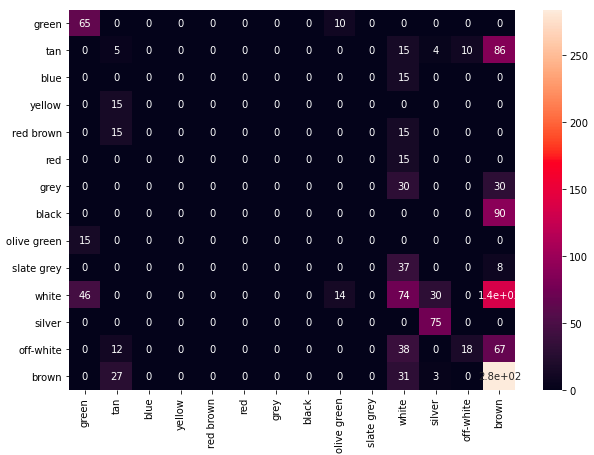
\includegraphics[scale=0.45]{latex/images/Heatmapbefore.png}
\label{fig:Heatmapbefore}
\caption{Predictions of color questions before training with new questions}
\end{figure}

\begin{figure}[H]
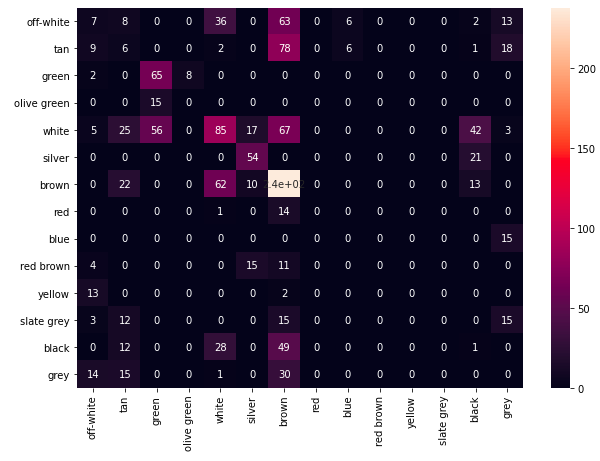
\includegraphics[scale=0.45]{latex/images/HeatmapAfter.png}
\label{fig:HeatmapAfter}
\caption{Predictions of color questions After training with new questions}
\end{figure}

\begin{figure}[H]
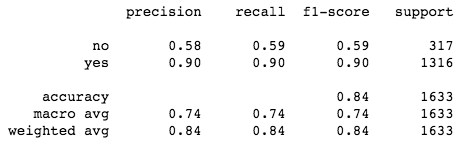
\includegraphics[scale=0.45]{latex/images/spatialscore.png}
\label{fig:HeatmapAfter}
\caption{Scores for spatial questions}
\end{figure}



\subsection{Discussion}

However, color questions could get more complex as "people employ compositional color descriptions to express meanings not covered by basic terms, such as greenish-blue" \cite{monroe2016learning}. It would be shallow to assume that color questions are simplistic, especially if we expect the system to answer colors beyond the basic color terms like "green" and "red." 

\cite{monroe2017colors}